\section{Memory and Experimental Conditions}
\label{app:methods}

\subsection{Consolidation Methods}

\begin{table}[h]
\caption{\textbf{Consolidation-method definitions.} ``Existing store access''
refers to whether the consolidator reads the current memory store before proposing an
update. \cond{SkillX} and \cond{Insights} are alternative consolidation
representations, whereas \cond{Schema Form-ED}, \cond{Schema Form}, and
\cond{Free Form} are LLM wiki variants.}
\label{tab:method-definitions}
\centering
\resizebox{\linewidth}{!}{%
\begin{tabular}{lllll}
\toprule
Method & Durable representation & Input grouping &
Existing store access & Organization / deduplication \\
\midrule
No Memory & none & none & no & none \\
No Consolidation & raw rollout & rollout & no & raw-rollout retrieval \\
SkillX & planning/functional/atomic skills & rollout independently & no &
three levels, no deduplication \\
Insights & strategy insight & rollout independently & no & flat, no deduplication \\
Schema Form-ED & typed wiki page & independent extraction then merge & merge step only &
fixed schema, deterministic matching \\
Schema Form & typed wiki page & sequential rollouts & yes &
fixed schema, implicit deduplication \\
Free Form & unconstrained wiki page & sequential rollouts & yes &
LLM-managed organization, implicit deduplication \\
\bottomrule
\end{tabular}}
\end{table}

Every row of the matrix in Table~\ref{tab:experiment-matrix} is run for
Claude Opus 4.6, GPT-5.4, and GLM-5 under the same benchmark, executor
loop, and task budget.

\begin{figure}[t]
\centering
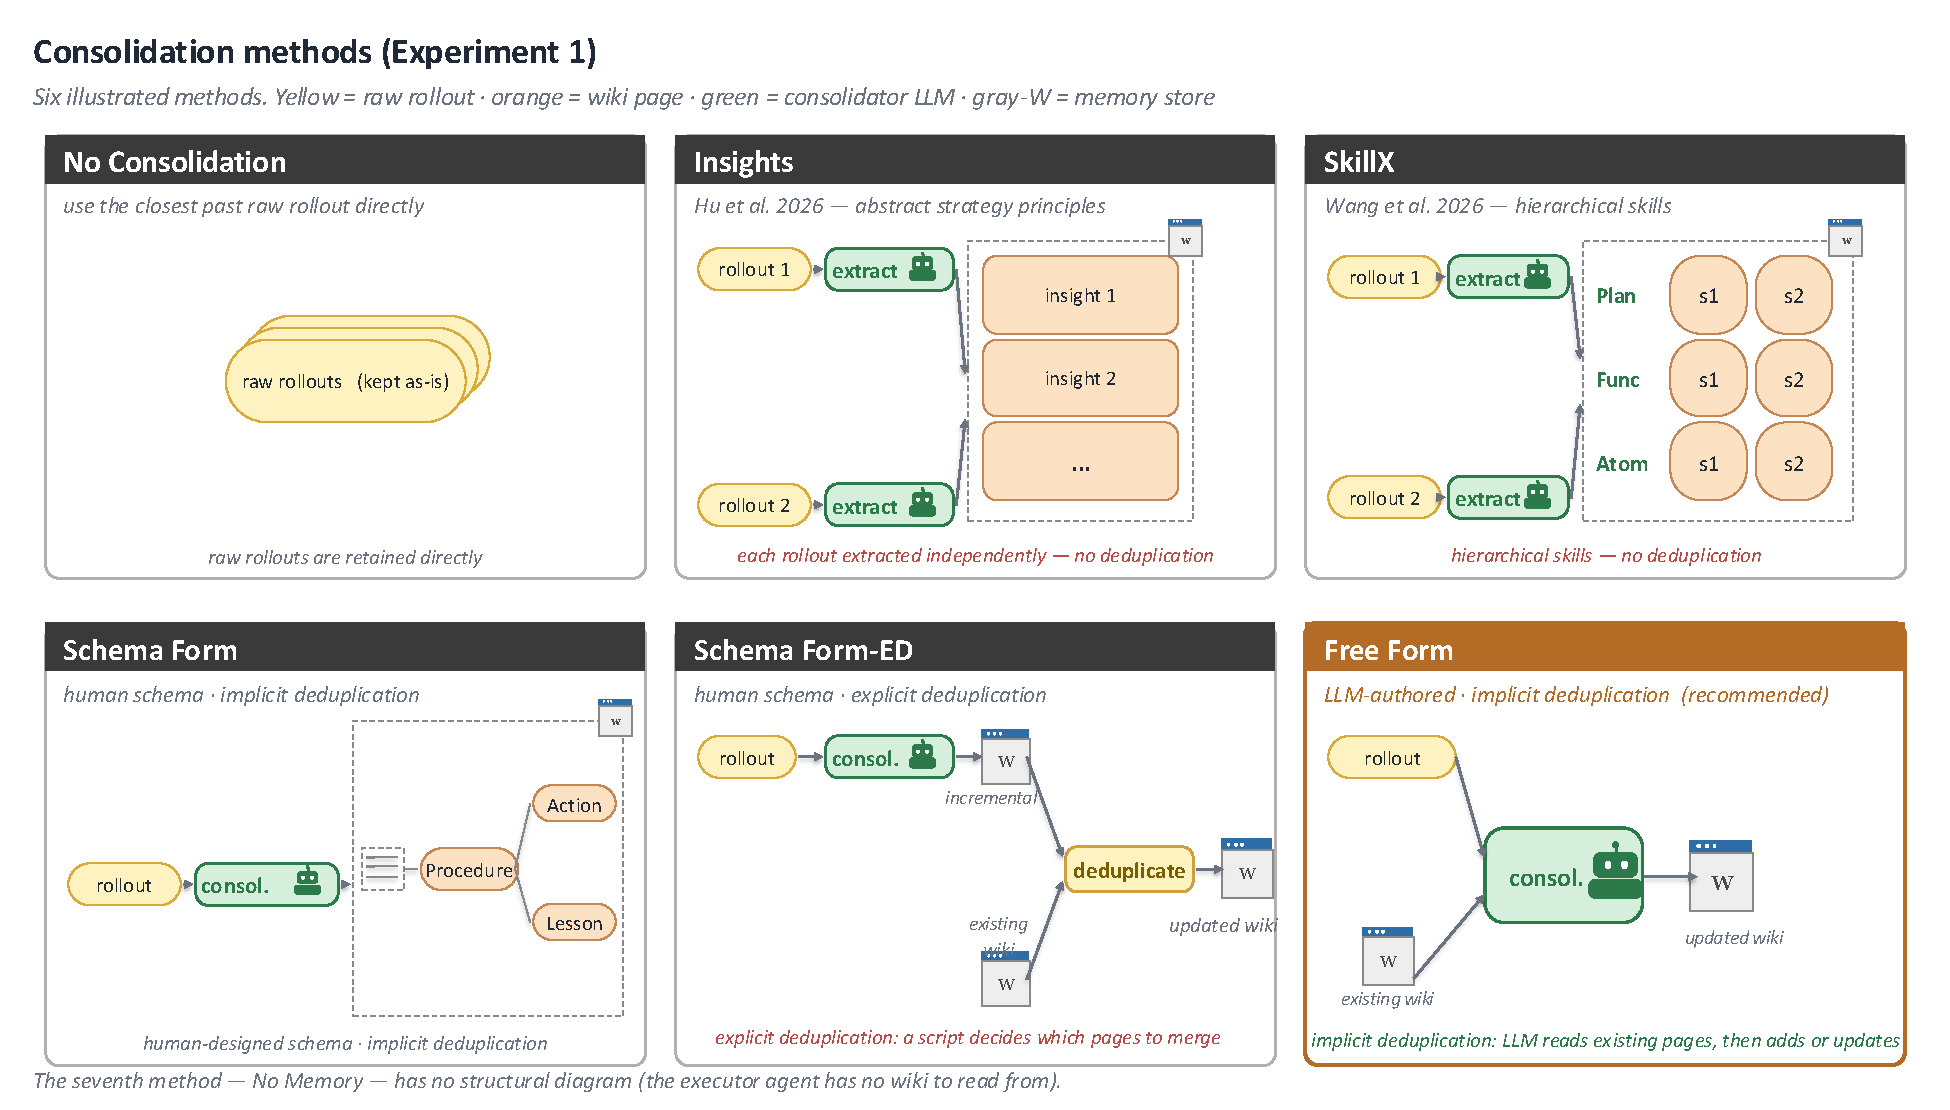
\includegraphics[width=0.92\linewidth]{fig_consolidation_methods.pdf}

\vspace{0.6em}
\begin{minipage}[t]{0.64\linewidth}
    \centering
    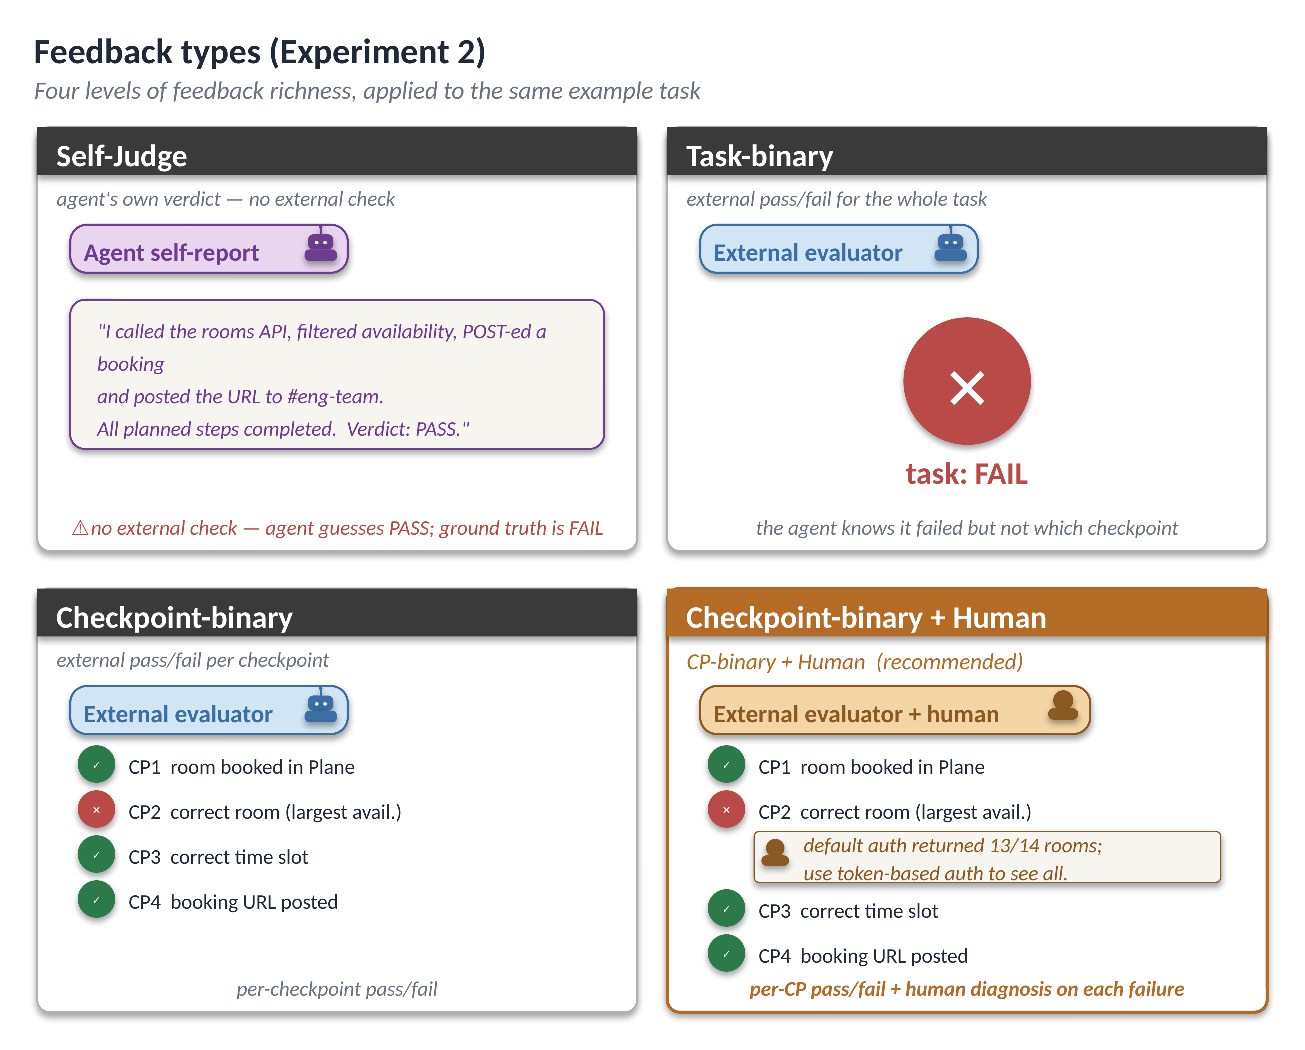
\includegraphics[width=\linewidth]{fig_feedback_types.pdf}
\end{minipage}\hfill
\begin{minipage}[t]{0.32\linewidth}
    \centering
    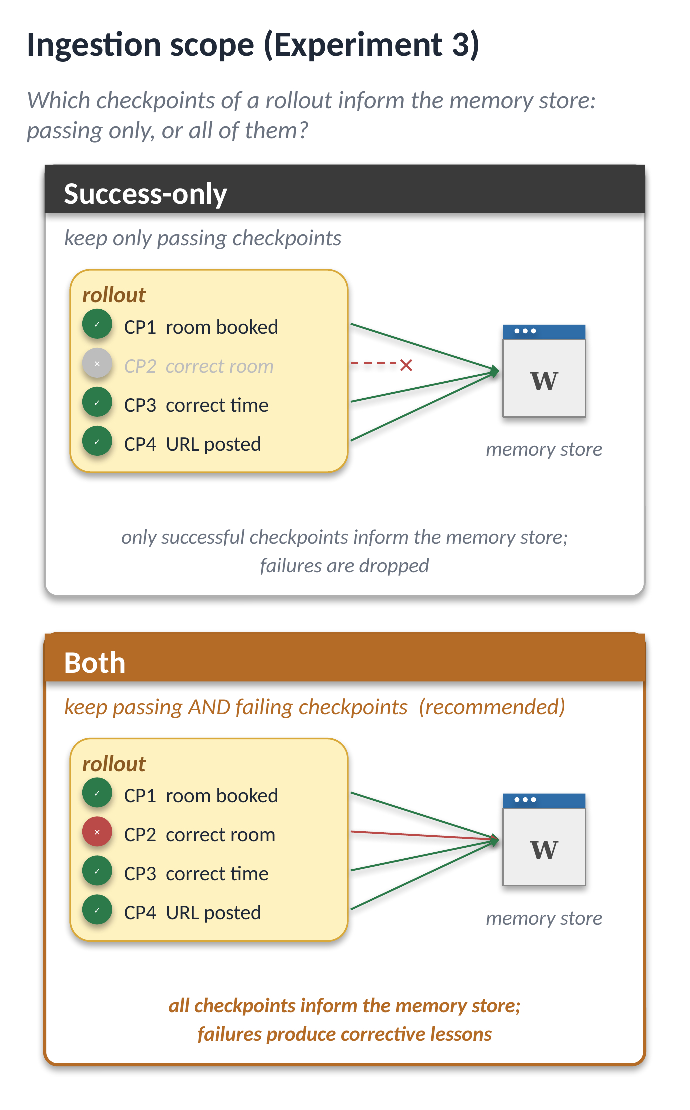
\includegraphics[width=\linewidth]{fig_ingestion_scope.pdf}
\end{minipage}
\caption{\textbf{Controlled procedural-memory design space.}
The consolidation methods varied in Experiment~1 appear above. Feedback
type (Experiment~2) and ingestion scope (Experiment~3) appear below at left and
right, respectively. The repeated workflow in Figure~\ref{fig:overview-workflow}
defines the round dimension in Experiment~4.}
\label{fig:overview-design}
\end{figure}

\paragraph{\cond{No Memory} and \cond{No Consolidation}.}
\cond{No Memory} executes without persistent experience. \cond{No Consolidation} stores raw
rollouts and retrieves the most similar one, testing whether experience replay
alone is sufficient.

\paragraph{\cond{Insights} and \cond{SkillX}.}
\cond{Insights} \citep{insights} independently extracts abstract strategy principles
from each rollout and gathers them in a flat store without cross-rollout
deduplication. \cond{SkillX} \citep{skillx} independently extracts planning,
functional, and atomic skills and organizes them by level, also without
cross-rollout deduplication.

\paragraph{LLM wiki variants.}
\cond{Free Form} lets the consolidator inspect the current wiki, then
decide what to record and whether to add a page or revise one. \cond{Schema Form} retains this one-step,
implicit deduplication process but requires three human-defined page types:
Procedures, Actions, and Lessons. \cond{Schema Form-ED}, short for Schema
Form with explicit deduplication, uses the same page schema but
first extracts incremental pages without seeing existing content. A
deterministic script then matches page identifiers and asks the LLM to execute
the selected merges.

\paragraph{Implicit and explicit deduplication.}
The two settings differ in who decides that a new page and an existing
page describe the same thing. Under \emph{implicit} deduplication, used by \cond{Free Form} and \cond{Schema Form}, consolidation is a single stage. The
consolidator sees the current wiki together with the new evidence. Deciding
whether that evidence
extends an existing page or warrants a new one is part of the same judgment
that writes the page. Under \emph{explicit} deduplication, used by \cond{Schema Form-ED}, consolidation is two stages. The consolidator first writes pages for
the new evidence with no sight of the current wiki, producing an incremental
wiki. A deterministic script then normalizes every page identifier and treats
two pages as duplicates when their normalized identifiers agree, for example
mapping any page describing a shell invocation of the Python interpreter to the
same action identifier regardless of what that invocation was for. Only the
selected pairs are passed back to the LLM, whose role is reduced to merging two
pages it is told belong together.

\paragraph{Page linking.}
Every wiki variant is reached from a single \texttt{index.md} entry
point and connected by Obsidian-style \texttt{[[wikilinks]]}, so that retrieval
can start at the index and walk to related content. The variants differ in what
the links are allowed to express. \cond{Free Form} places links wherever the
consolidator judges two pages related, and the resulting graph is unconstrained.
The two schema variants inherit a fixed link grammar from the page types: a
Procedure links to every Action it invokes, and a Lesson attaches to the single
Procedure or Action whose failure it describes. Actions do not link to one
another, so a procedure's steps are recoverable only through the Procedure page
that lists them. Table~\ref{tab:qualitative-filter} records a related
omission, a schema page that names a step without the detail needed to execute
it.

\subsection{Memory Organization by Method}

\paragraph{\cond{No Consolidation}: raw rollout store.}

\paragraph{\cond{Insights}: flat insight set.}

\paragraph{\cond{SkillX}: three skill tiers.}

\paragraph{\cond{Schema Form} and \cond{Schema Form-ED}: typed wiki pages.}

\paragraph{\cond{Free Form}: unconstrained LLM wiki.}

\subsection{Execution Process}

\paragraph{Executor loop and task budget.}

\paragraph{How retrieved memory enters the executor context.}

\paragraph{Termination and what a rollout record contains.}

\subsection{Consolidation and Retrieval Protocols}

\paragraph{Consolidation execution.}
All task executions within round $r$ use the frozen store $M_r$. After
evaluation, the eligible rollouts, meaning those the ingestion scope
admits, are enumerated in lexicographic filename order.
\cond{Free Form} and \cond{Schema Form} process them sequentially against a mutable copy of
$M_r$, so each successful update is visible when processing subsequent
rollouts. \cond{Insights} and \cond{SkillX} process each rollout independently, potentially
in parallel, without access to other extracted outputs. \cond{Schema Form-ED}
independently extracts candidate pages, applies deterministic matching, and
invokes the LLM for selected merges. After all eligible rollouts are processed,
the semantic index over the store is rebuilt to produce $M_{r+1}$.

\paragraph{Retrieval execution.}
Each condition runs its retrieval stage before planning. \cond{No Memory} omits
retrieval, and \cond{No Consolidation} supplies the retrieved
raw-rollout trace. For
consolidated representations, a retrieval-only agent receives the task
instruction and a read-only memory path in a fresh session. It may search the
representation-specific semantic index, inspect the representation's index or
routing file, and read selected files in full, but it cannot interact with the
task environment. If task-level retrieval finds no matched memory, the agent
may search again for each \emph{subgoal}, meaning one step of the plan
the executor has formed. An execution failure also
triggers a fresh subgoal search. Table~\ref{tab:retrieval-adapters} summarizes the
adapter-specific search and expansion rules.

\begin{table}[h]
\caption{\textbf{Representation-specific retrieval adapters.} The executor
loop is shared, while each adapter exposes the native organization of its
memory representation. ``Search'' is semantic search over file contents,
and ``index'' and ``routing'' are the representation's own entry-point file.}
\label{tab:retrieval-adapters}
\centering
\resizebox{\linewidth}{!}{%
\begin{tabular}{llll}
\toprule
Representation & Task-level retrieval & Subgoal retrieval & Context expansion \\
\midrule
No Memory & none & none & none \\
No Consolidation & raw-rollout retrieval & none & retrieved rollout trace \\
Insights & search/index, up to 5 files & search, up to 3 files & full insight files \\
SkillX & search/routing, up to 5 files & search/routing, up to 3 files &
full files across skill tiers \\
Schema variants & top procedure from 3 candidates & top 5 actions per query &
linked procedures, actions, and lessons \\
Free Form & search top 5 per query/index & search/index, up to 3 pages &
full wiki pages \\
\bottomrule
\end{tabular}}
\end{table}

\paragraph{Retrieval walkthrough for each method.}

\subsection{Feedback Type, Ingestion Scope, and Rounds}

\begin{table}[h]
\caption{\textbf{Feedback types.} Rich feedback denotes \cond{Checkpoint-binary + Human}, and weak feedback denotes \cond{Self-Judge}.}
\label{tab:feedback-definitions}
\centering
\small
\begin{tabularx}{\linewidth}{@{}lX@{}}
\toprule
Feedback type & Information available during consolidation \\
\midrule
Self-Judge & Agent self-assessment without an external outcome signal. \\
Task-binary & External pass/fail for the whole task. \\
Checkpoint-binary & External pass/fail for each checkpoint. \\
Checkpoint-binary + Human & Checkpoint outcomes plus human failure diagnosis. \\
\bottomrule
\end{tabularx}
\end{table}

\cond{Success-only} selects evidence associated with passed checkpoints. \cond{Both}
(successes and failures) selects evidence from all checkpoints. One round is one execute phase over all
benchmark tasks followed by one consolidate phase. R0 has no memory
store, while R1 to R4 execute with and then update the persistent store
produced previously.

\subsection{Controlled Experimental Matrix}

\begin{table}[h]
\caption{\textbf{Controlled experimental matrix.} Each experiment varies one
focal dimension while fixing the remaining dimensions.}
\label{tab:experiment-matrix}
\centering
\resizebox{\linewidth}{!}{%
\begin{tabular}{llllll}
\toprule
Experiment & Varied dimension & Method & Feedback & Scope & Rounds \\
\midrule
1 & Consolidation method & seven conditions &
Checkpoint-binary & Both & R1 \\
2 & Feedback type & Free Form &
four conditions & Both & R1 \\
3 & Ingestion scope & Free Form &
Self-Judge and Checkpoint-binary + Human & Success-only, Both & R1 \\
4 & Rounds & Free Form &
Self-Judge and Checkpoint-binary + Human & Both & R0 to R4 \\
\bottomrule
\end{tabular}}
\end{table}

\subsection{Consolidation Prompts}
